\section{Overview}

Machine learning is a sub-field of data analytics that uses semi-automated techniques to transform data into insights. Machine learning plays a major role in the modern world and forms the backbone for everything from image recognition \citep{Davis2018Real-TimeDrones} to weather forecasting \citep{McGovern2017UsingWeather}. Today, there are thousands of different machine learning techniques that fall into a number of major categories. In this work, we are primarily interested in paradigm of supervised learning.

In its most simplistic form, \textit{supervised learning} is the art of fitting functions to data. Given some known input vector $x$ and an unknown response vector $y$, we would like to make a well-founded approximation of what that output vector is likely to be, $\hat{y}$. Ideally, this output $\hat{y}$ should be guided by how the inputs and the outputs have interacted in the past. While there are many different techniques for generating this prediction, most methods have three features in common: a function approximator, a loss function, and an optimizer. 
   
Supervised models rely on the assumption that the outputs can be described as some function of the inputs $f(x)$ plus some unpredictable element $\sigma$, known as \textit{noise} (equation \ref{eq:simple_model}). 

\begin{equation}
    \label{eq:simple_model}
    y = f(x) + \sigma
\end{equation}

A \textit{function approximator} does its best to mimic this underlying function without getting thrown off by the noise. Different techniques implement this approximator in different ways, and each technique has its advantages and drawbacks.

Just as important as the function approximator is the \textit{optimizer}, which determines how the approximator will learn from the data and how it will handle noise. A key element of an optimizer is the \textit{loss function}, which measures the difference between a model’s output and the actual output, a value known as the \textit{residual}. The optimizer is the most important feature during model training, and more powerful approximators typically have more complex optimizers. 

Two important features to consider when designing a model are its power and interpretability. \textit{Power} describes how well the approximator can describe arbitrarily complex behavior, while \textit{interpretability} describes how easy it is for a human to understand how the model came to its conclusion. More powerful models are more capable of approximating the underlying function, but are generally less interpretable \citep{Du2018TechniquesLearning}. 

\section{Linear Regression and Elastic Nets}

Linear regression is the oldest and possibly simplest form of machine learning. The function approximator is a simple weighted sum of the input variables plus a bias (equation \ref{eq:linear_regression}).

\begin{equation}
    \label{eq:linear_regression}
    \hat{y} = w \cdot x + w_0 = \sum_{i=1} ^ {n} {w_i x_i} + w_0
\end{equation}

The most common loss function minimizes the sum of the squares of the residuals. This squaring has the effect of amplifying large residuals, forcing the model to account more heavily for outliers. In its most basic form, linear regression with this type of loss function is known as ordinary least squares regression (equation \ref{eq:linear_regression_loss}). 

\begin{equation}
    \label{eq:linear_regression_loss}
    loss = (\hat{y} - y) ^ 2
\end{equation}

This loss function has the added benefit in that it is analytically tractable, a unique feature among machine learning methods making ordinary least squares a highly efficient machine learning method. The weights that minimize this loss function can be found using the following equation (equation \ref{eq:linear_regression_optimize}).

\begin{equation}
    \label{eq:linear_regression_optimize}
    \hat{w} = (x^\top x) ^ {-1} (x^\top y)
\end{equation}

Computationally cheap and remarkably effective, linear regression has been a benchmark of statistics since the late 19th century \citep{Galton1886RegressionStature.}. While useful in a number of applications, simple linear regression does have drawbacks that limit its usefulness in many scenarios.

The first issue with simple linear regression is that it tends to overfit when presented with a large number of features relative to the number of samples. This issue can be mitigated by adding a \textit{regularizer} that penalizes large weights. The two most common regularization techniques are to punish on the absolute value of the weight, or $L_1$ norm \citep{Santosa1986LinearSeismograms}, and to punish on the  squared value of the weight, or the $L_2$ norm \citep{Tikhonov1977SolutionsProblems}. Linear regression that employs just the $L_1$ punishment is called \textit{Lasso Regression} \citep{Tibshirani1994RegressionLasso}, just the $L_2$ punishment is called \textit{Ridge Regression}, and the technique that employs both punishments is called an \textit{Elastic Net} \citep{Zou2005RegularizationNet}. Each regularizer is weighted with a hyper-parameter that must be tuned during validation. Because elastic nets use two regularizers, the technique requires tuning of two hyper-parameters. 

While regularizers can help solve the over-fitting issue, linear models still have limitations on the type of functions they can model. Most importantly, linear regression assumes that the underlying output variable can be represented as a simple linear combination of the inputs, something that’s just not true for most real-world problems. 

\section{Tree-Based Methods}

In order to model non-linear functions, we need to move away from simple linear regression, towards more powerful techniques. Decision trees are one of the oldest non-linear machine learning methods \citep{Breiman1984ClassificationTrees}, and variations on the technique are still common to this day \citep{Natekin2013GradientTutorial}. 

Similar to a flowchart, decision trees work by iteratively asking a sequence of yes/no questions that move the model towards a prediction (see Figure \ref{fig:decision_tree_example}). This process segments the input space, effectively grouping elements that are perceived to be similar or share important characteristics. The model then takes an average of the output of these grouped elements. While initially fit by hand \citep{Chisholm1968TheHumidity}, \update{decision trees became a staple of machine learning with the development of} an optimizer that could algorithmically determine variable splits using training data \citep{Breiman1984ClassificationTrees}.

\begin{figure}
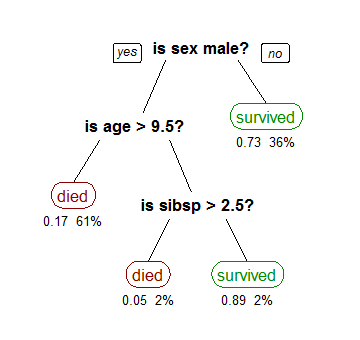
\includegraphics[width=0.65\textwidth]{fig/decision_tree_example.png}
\centering
\caption{Example of a decision tree trained on the Titanic dataset (see below). Trunk nodes represent decisions to be made and leaf nodes represent the final prediction.}
\label{fig:decision_tree_example}
\end{figure}

This optimizer works in a greedy, top-down fashion, iteratively splitting the input space and calculating an impurity metric. While many such metrics exist, such as Gini impurity \citep{Breiman1984ClassificationTrees}, information gain \citep{Kullback1951OnSufficiency}, and variance reduction \citep{Breiman1984ClassificationTrees}, they all effectively work to minimize the dissimilarity of the response variable in each group. When the branch with the smallest impurity is found, the tree splits on that variable and the process is repeated recursively for the two new groups. 

The adoption of the decision tree was a significant step forward for the field of machine learning. Unlike linear regression, which is restricted to the realm of linear functions, decision trees can approximate any rational function. However, this assertion comes with an important caveat. Because decision trees are discrete entities, they require a large number of splits to accurately approximate continuous functions. 

\begin{figure}[t]
\caption{Approximating a continuous sigmoid function with decision trees of varying depths. Greater depths provide better precision but also require more data to train.}
\includesvg[width=0.65\textwidth]{fig/decision_trees.svg}
\centering
\end{figure}

Every split approximately halves the number of data points in each bin, quickly burning through all available information and causing the method to overfit. As a result, the depth of decision trees must be kept low, making them more “brittle” and causing them to give poor estimates near the decision boundaries. 

One solution to this issue is to ensemble many trees together, with each tree fit to a slightly different version of the data. This method is known as random forest regression \citep{Ho1995RandomForests}. Random forests employ two techniques to augment the data before training a tree: bootstrapping \citep{Ho1995RandomForests} and bagging \citep{Ho2002AConstructors}. Bootstrapping randomly samples $n$ points from the data with replacement while bagging takes a random sub-sample of the features. These modifications weight the data just enough to break symmetry and develop a large number of independent, predictive trees. By averaging the output of these trees, random forests create a smoother function without needing to add additional depth. 

\begin{figure}
\caption{Approximating a continuous sigmoid function with a random forest of depth 2. Compared to decision trees of similar depth, the random forest provides much smoother, and therefore more accurate predictions of the underlying function without requiring additional training data.}
\includesvg[width=0.65\textwidth]{fig/random_forest.svg}
\centering
\end{figure}

One further improvement to random forests is the Gradient Boosted Machine (GBM) \citep{Friedman2001GreedyMachine}. A sort of addition to random forests, GBMs add weight to misclassified samples during training, causing future trees to focus more heavily on difficult regions in the solution space. This modification can often increase performance, by refocusing the model's power on difficult-to-model regions, even if there are relatively few samples in that area. The downside though, is that the trees must be trained sequentially rather than in parallel, slowing the time it takes to fit a model. 

Note that each improvement on the standard decision tree decreases the model's overall interpretability. Where decision trees can be read like a flowchart, random forests are an average of lots and lots of trees, making it more difficult to parse out every combination of outcomes. On the other hand, random forests have a very clear-cut notion of variable importance, with more common splits being more important to the outcome. This analysis is somewhat more difficult in GBMs due to the non-trivial nature of how the samples are weighted before each tree is trained.  

\section{Artificial Neural Networks}

Another powerful machine learning technique is the artificial neural network. Neural networks are a modular approach to function approximation. The base unit is a weighted sum fed in to a non-linear activation function called a \textit{perceptron}.

\begin{figure}
\caption{An example of a perceptron with inputs $x_1$ and $x_2$ and a step function activation. The bias is represented by $w_0$ and the output is represented by $\gamma$.}
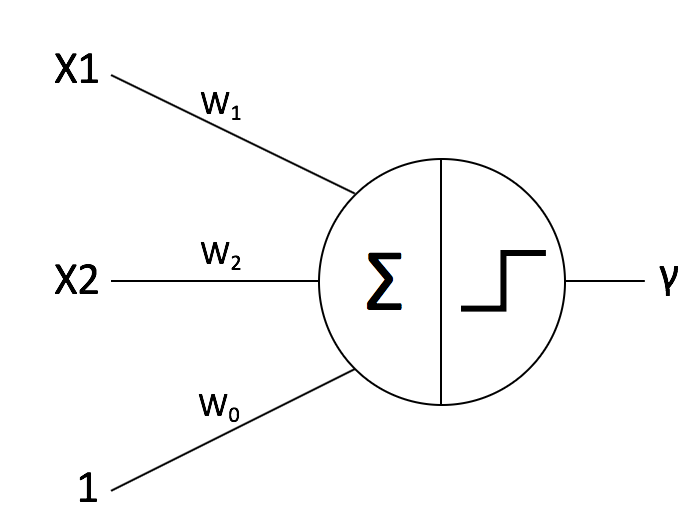
\includegraphics[width=0.65\textwidth]{fig/perceptron}
\centering
\end{figure}

To get the output of a perceptron, the inputs plus a bias are weighted according to vector $w$. These weighted values are then summed together and fed as the input to a non-linear activation function $f$. The purpose of this activation is to allow the perceptron to expand beyond linear functions. Many different activations exist, and the optimal choice is still a point of open research \citep{Duch2000TaxonomyFunctions} \citep{Xu2015EmpiricalNetwork}. Historically, the most common activation function has been the sigmoid \citep{Minsky1969PerceptronsGeometry} but there is increasing interest in other activations, including the rectified linear unit \citep{Glorot2011DeepNetworks}, the leaky-rectified linear unit \citep{Maas2013RectifierModels}, and the exponential linear unit \citep{Clevert2015FastELUs}. 

While potentially more powerful than linear regression, the perceptron is still highly limited in the types of functions it can approximate. For instance, the output of a single perceptron with sigmoid activation will always be sigmoidal. We can get around this limitation by stacking many perceptrons together in parallel. In fact, it has been proven \citep{Cybenko1989MathematicsFunction} that a weighted sum of a large number of perceptrons can approximate any rational function. This mesh of perceptrons is known as a \textit{neural network} and has three layers: one input layer containing the features, one output layer containing the predictions, and at least one hidden layer containing the perceptrons. 

However, while possible to approximate any rational function with this architecture, it is not always easy to do so. Complex functions often require a large number of hidden nodes, which in turn require large amounts of data and computational resources. One remedy for this issue to stack multiple perceptron layers one after the other \citep{Rumelhart1985LearningPropagation}, allowing each layer of the network to learn simpler functions which generalize more effectively, before combining them together into the full result (see Figure \ref{fig:deep_network}). This effect can speed network convergence, reduce training time, and can radically increase accuracy without requiring additional data. 

\begin{figure}[ht]
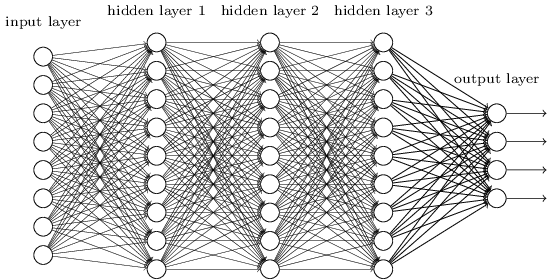
\includegraphics[width=0.65\textwidth]{fig/deep_network.png}
\centering
\caption{Example of a muli-layer neural network. Each node in the graph represents a summation and an activation, which each edge represents a weight. Image credit \cite{Nielsen2015NeuralLearning}.}
\label{fig:deep_network}
\end{figure}

In high-dimensional input spaces where input proximity is meaningful (images or speech for instance) further improvements can be achieved through the use of \textit{convolutions} \citep{Fukushima1980Neocognitron:Position}. A convolutional network runs a sequence of filters over an image to create the inputs for the next layer. While less powerful than a traditional dense layer, this technique significantly reduces the total number of connections by ensuring that only spatially-related information is included in the transformation. This reduction allows convolutional networks to effectively train more complex structures on less input data.

Networks with a large number of convolutional or dense layers are known as \textit{deep networks}, and have produced state-of-the-art results in long-standing computational challenges, including image recognition \citep{Davis2018Real-TimeDrones}, machine translation \citep{Bahdanau2014NeuralTranslate}, and weather forecasting \citep{McGovern2017UsingWeather}. 

Unlike logistic regression, which is analytically tractable, and decision trees, which have a linear-time algorithm for determining splits, artificial neural networks are trained using the \textit{gradient descent algorithm}. Mathematically, the objective of gradient descent is to minimize a loss function, which for simplicity, we will consider to be the sum of the squared residuals as in linear regression (equation \ref{eq:mse_loss}). 

\begin{equation}
    \label{eq:mse_loss}
    loss = \sum_{i=0}^{n}{(y_i-\hat{y_i})^2}
\end{equation}

Because there does not exist an analytical solution to this optimization problem, we are forced to use numerical methods to approximate a solution. By relating the weights of the network to the loss function and computing a derivative, it is possible to determine which way to adjust the weights to lower the overall error of the network (equations \ref{eq:part_loss} and \ref{eq:back_prop}).

\begin{equation}
    \label{eq:part_loss}
    loss_i = (y_i-f(w^\top x))^2
\end{equation}

\begin{equation}
    \label{eq:back_prop}
    \frac{\partial_{loss_i}}{\partial_{w_j}} = -2 (y_i - f(w^\top x)) f'(w^\top x) x_j
\end{equation}

A similar formula can be derived for deeper layers by invoking additional iterations of the chain rule. By iteratively pushing the weights a small amount, the network reduces in error until it reaches an equilibrium state, in which it is considered \textit{fit} to the data. 

With the success of the deep learning paradigm, neural networks have become ubiquitous in the field of machine learning. Powerful libraries including Keras \citep{Chollet2019Keras}, TensorFlow \citep{Martin2015TensorFlowSystems}, and PyTorch \citep{Paszke2017AutomaticPyTorch}, make it easy to train and integrate neural networks on a range of systems and hardware. TensorFlowJS \citep{TensorFlow2019TensorFlow.js} allows neural networks to be embedded in web frameworks while other extensions provide support for statistical software like R \citep{Allaire2019RTensorFlow}. Years of research in the field have developed highly efficient methods and optimizers to train networks faster on larger amounts of data \citep{Kingma2014Adam:Optimization}. These successes and widespread support have made neural networks one of the most common methods for modeling in industry, spanning fields from weather forecasting \citep{Lagerquist2017MachineWind} to ecology \citep{Chilson2019AutomatedNetworks}. 

Like random forests and GBMs, neural networks suffer from a lack of interpretability. While architecture-specific improvements have been suggested to simplify \citep{Olden2002IlluminatingNetworks} or visualize \citep{Ozesmi1999AnInteraction} the transformations inside a network, none of these solutions fully resolve the interpretability issue. As a result, researchers have started looking to other tools to help explain a model's output.

\section{Local Approximation}

One important interpretability technique is to approximate a model over a small domain rather than approximating the entire function. In other words, our objective is to fit a linear model such that it is a faithful representation of the larger model on some domain. This approach works well, as most models behave linearly on a small enough scale, allowing for relatively simple interpretations. 

The most obvious local linear approximator is a first-order Taylor polynomial centered at a desired point. This approach simply fits a line to the slope of the model at a given point. While this technique works, it can be extremely misleading. Taylor polynomials are only guaranteed to be accurate when very close to initial point, which may not be a good indicator of what the model is doing on a more reasonable interval. 

\begin{figure}[t]
    \centering
    \caption{Example of Taylor Polynomials failing to approximate the neighborhood behavior of a non-linear function. \citep{Plumb2019RegularizingInterpretability}}
    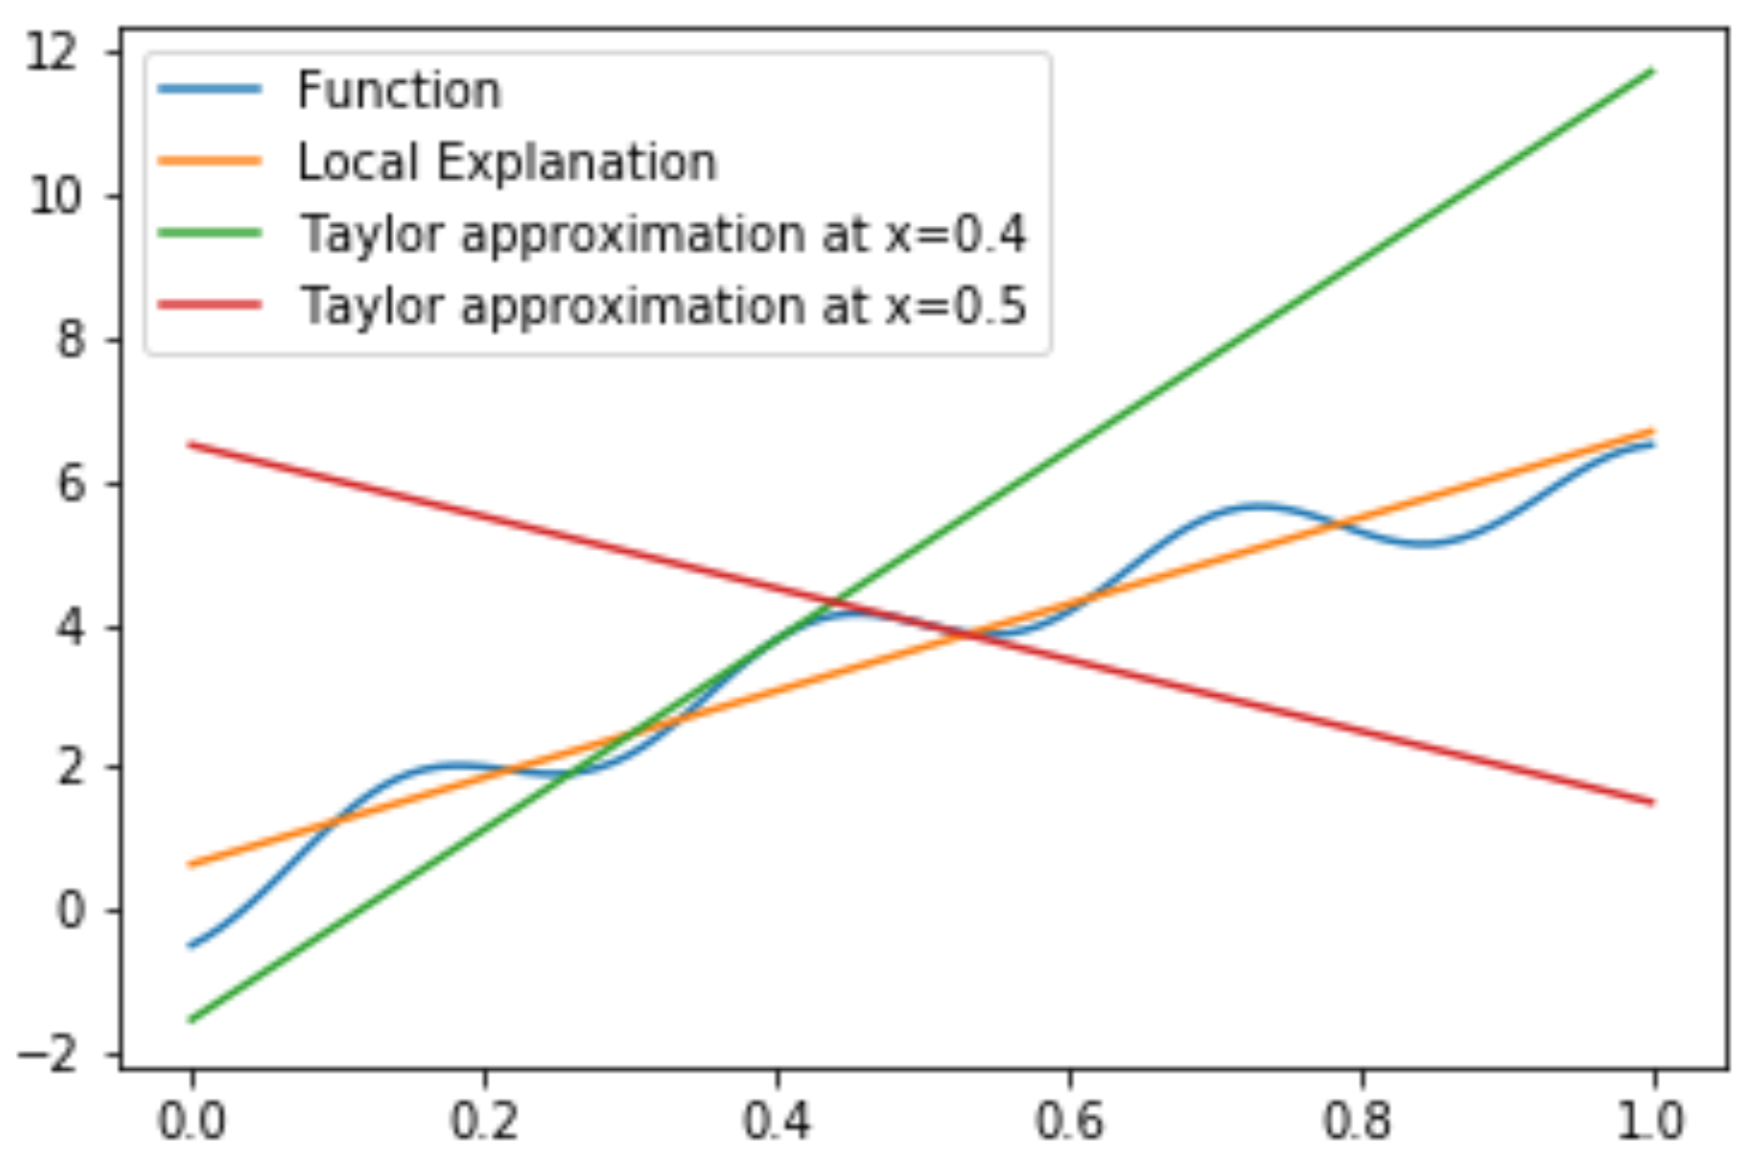
\includegraphics[width=0.65\textwidth]{fig/taylor_polynomial}
    \label{fig:taylor_polynomial}
\end{figure}

A better approach is to fit a linear model over a neighborhood that can be defined by the investigator. This linear model will be more stable than the Taylor approximation, and will provide better approximations, so long as the neighborhood selected is guaranteed to be approximately linear. While there are different ways of addressing this problem, one approach is to apply regularizers to the model during training, guaranteeing the model to be approximately linear in some neighborhood \citep{Plumb2019RegularizingInterpretability}.

Local approximation techniques are still an open area research \citep{Ribeiro2016WhyClassifier, Plumb2018ModelExplanations} and initial results have been promising. However, these approaches only cover local approximations. In large input spaces, it is infeasible to test every potential point for a local approximation, so we instead look to other methods to explain the global behavior of an arbitrary model. 

\section{Global Approximation Methods}

Partial dependence plots (PDP) and Individual Conditional Expectation (ICE) are two of the most popular model-agnostic methods for interpreting the global behaviors of machine learning methods. Both work by varying one input $x$ across its full range of possible values while holding all other inputs constant and plotting the response. In ICE this process is repeated for each data point and all plots are shown. In PDP, the mean response is plotted for each value of $x$. While these techniques do work, they are far from perfect. 

\begin{figure}[t]
    \centering
    \caption{Example of a PDP plot layered on top of an ICE plot. Black lines represent ICE and the thick yellow line represents the PDP plot. \citep{Molnar2019InterpretableLearning}}
    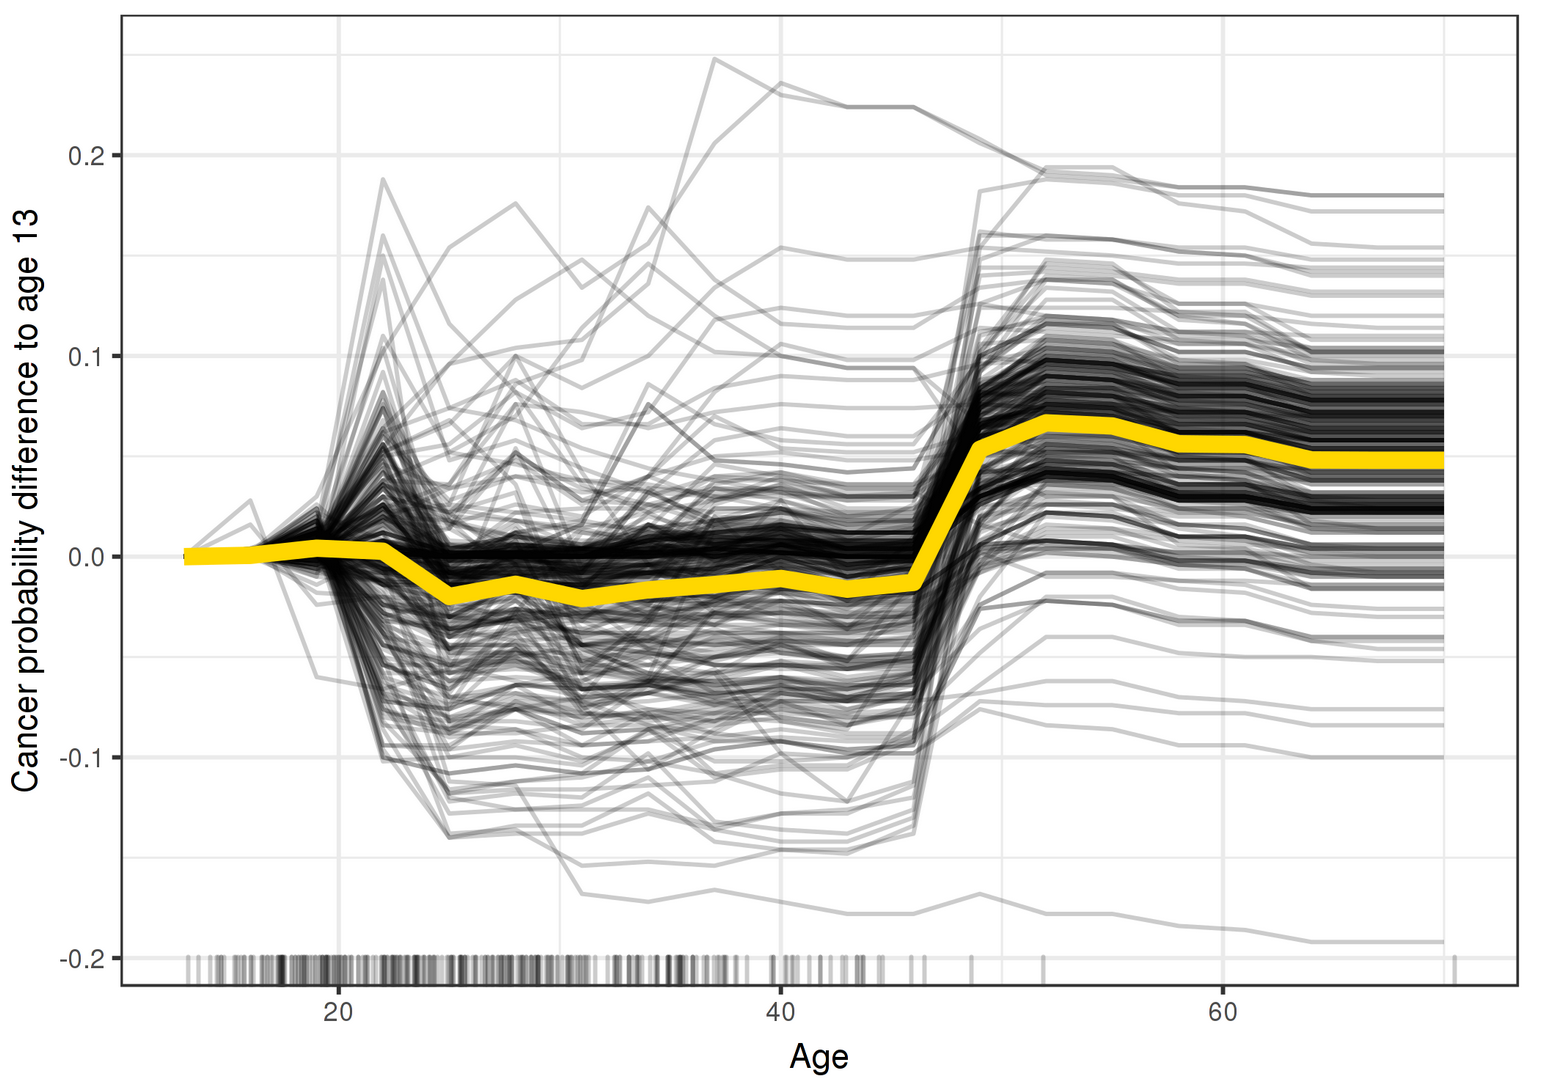
\includegraphics[width=0.65\textwidth]{fig/ice}
    \label{fig:ice}
\end{figure}


ICE plots track every observation across the range of all possible values $x$. While fine for a small sample, as the number of observations grow, ICE plots become more complex and difficult to read. While sub-sampling can help with this complexity, it runs the risk of leaving out important behaviors. Furthermore, in ICE plots its often unclear which line correlates with observation, somewhat dampening the overall interpretability. 

PDP plots suffer from the opposite issue. While simple and easy to read, they rely on several strong assumptions which can lead to poor approximators for the underlying model. The most important assumption for PDP plots is the that of input independence, as correlations in the input space will result in unrealistic values being included in the average. For instance, a PDP plot investigating the impact of input $x_1$ on output $E(y|x_1, x_2)$ will provide biased results if $x_1$ and $x_2$ are highly correlated, as some values of $x_2$ will be significantly less likely given a known value of $x_1$, but will still be included in the PDP average. Furthermore, because they take an average of a set of observations, PDP plots do not address the impact of joint terms in the model, and therefore miss a significant portion of model behavior. 

Finally, neither method describes how the model will extrapolate to under-defined regions in the input space. For instance, if our underlying function is $y = x_1 x_2^2$ and we’re looking at an ICE plot of $x_2$, where we have only seen large positive and negative values of $x_1$, the figure will contain two parabolic structures, one for positive values of $x_1$ and one negative values. While useful for known values, the plot provides no information on what the model would do if $x_1$ were equal to zero. 

\begin{figure}
\centering
\begin{subfigure}{.5\textwidth}
  \centering
  \includesvg[width=0.9\linewidth]{fig/bkg/dot_custom.svg}
  \caption{Dot plot of variable $x_2$.}
\end{subfigure}%
\begin{subfigure}{.5\textwidth}
  \centering
  \includesvg[width=0.9\linewidth]{fig/bkg/ice_custom.svg}
  \caption{Joint ICE and PDP plot of variable $x_1$.}
\end{subfigure}
\caption{Example of how ICE/PDP plots can lead to deceptive results in under-defined input regions. In this instance, $x_2$ is distributed bimodally, with peaks at positive and negative five. These peaks correspond to two sets of parabolic curves in the ICE plot and a trivial PDP curve. Aside from the PDP plot being unhelpful, the dot and ICE plots strongly suggest that the behavior of $x_1$ is stable on the interval [-8,8]. However, an unexpected inverse causes outlier point one (red) to exhibit aberrant behavior. Actual function: $y = \frac{-x_1^2 + 0.25}{x_2}$}

\label{fig:custom}
\end{figure}

This blind spot is a major issue in real-world applications, as under-defined regions are the most likely to break a well-fit model in a live environment. 

The fundamental issue with each of these methods is that there is no feasible two-dimensional representation sufficient to explain the complexity of an arbitrary machine learning model. While possible to generalize the behavior to some degree, there is always a risk of encountering some portion of the input space that was not covered by the interpretation scheme. 

One solution is to simplify the model itself, such that the internal representations can be expressed exactly as a PDP plot, or a simple sum of arbitrary one-dimensional functions. While uncommon in machine learning, this approach is well-known in the field of statistics as a \textit{Generalized Additive Model} (GAM). 

\section{Logistic Regression, GLMs, and GAMs}

Before jumping in to GAMs, we first need to explore an important early development in the linear paradigm: logistic regression \citep{Nelder1972GeneralizedModels}. Linear regression has a number of drawbacks, but one of the most troublesome was the lack of support for classification problems. This issue with this class of problem is that the response always takes one of two values: zero or one. This feature violates the constant variance assumption of linear regression and leads to impossible behaviors, such as predictions with over one-hundred or below zero percent confidence. 

Logistic regression solves this issue by piping the output from linear regression into a sigmoid (equation \ref{eq:sigmoid}, bounding the predictions between zero and one. This simple step was a major breakthrough, as it proved that linear models could be expanded beyond linearly structured problems. 

\begin{equation}
    \label{eq:sigmoid}
    \frac{\partial_{loss_i}}{\partial_{w_j}} = -2 (y_i - f(w^\top x)) f'(w^\top x) x_j
\end{equation}

Similar approaches were applied using other distributions, allowing the distribution of the response to take the form of a Poisson or Bernoulli, for instance. Methods of this type are known as \textit{Generalized Linear Models} \citep{Nelder1972GeneralizedModels} and use a \textit{link} function to circumvent the constant variance assumption of linear regression. 

Further improvements can be attained using Generalized Additive Models (GAMs) \citep{Hastie2007GeneralizedModels} which take the additional step of delinearizing each of the inputs as well as outputs. This change significantly improves the predictive power of the model, allowing it to handle complex non-linear functions nearly as well as other machine learning techniques like random forests or neural networks. 

GAMs work by passing each of the inputs through carefully selected \textit{spline} functions, which delinearize the inputs before passing them into the model. By combining multiple non-linear functions together the model can effectively approximate arbitrary combinations of non-linear behavior as illustrated in Figure \ref{fig:fancy_spline}. This technique is effectively a form of feature engineering which significantly increases our input space \citep{Molnar2019InterpretableLearning}. GAMs therefore employ a regularizer similar to elastic nets which help dampen the weights to prevent over-fitting.

\begin{figure}[t]
    \centering
    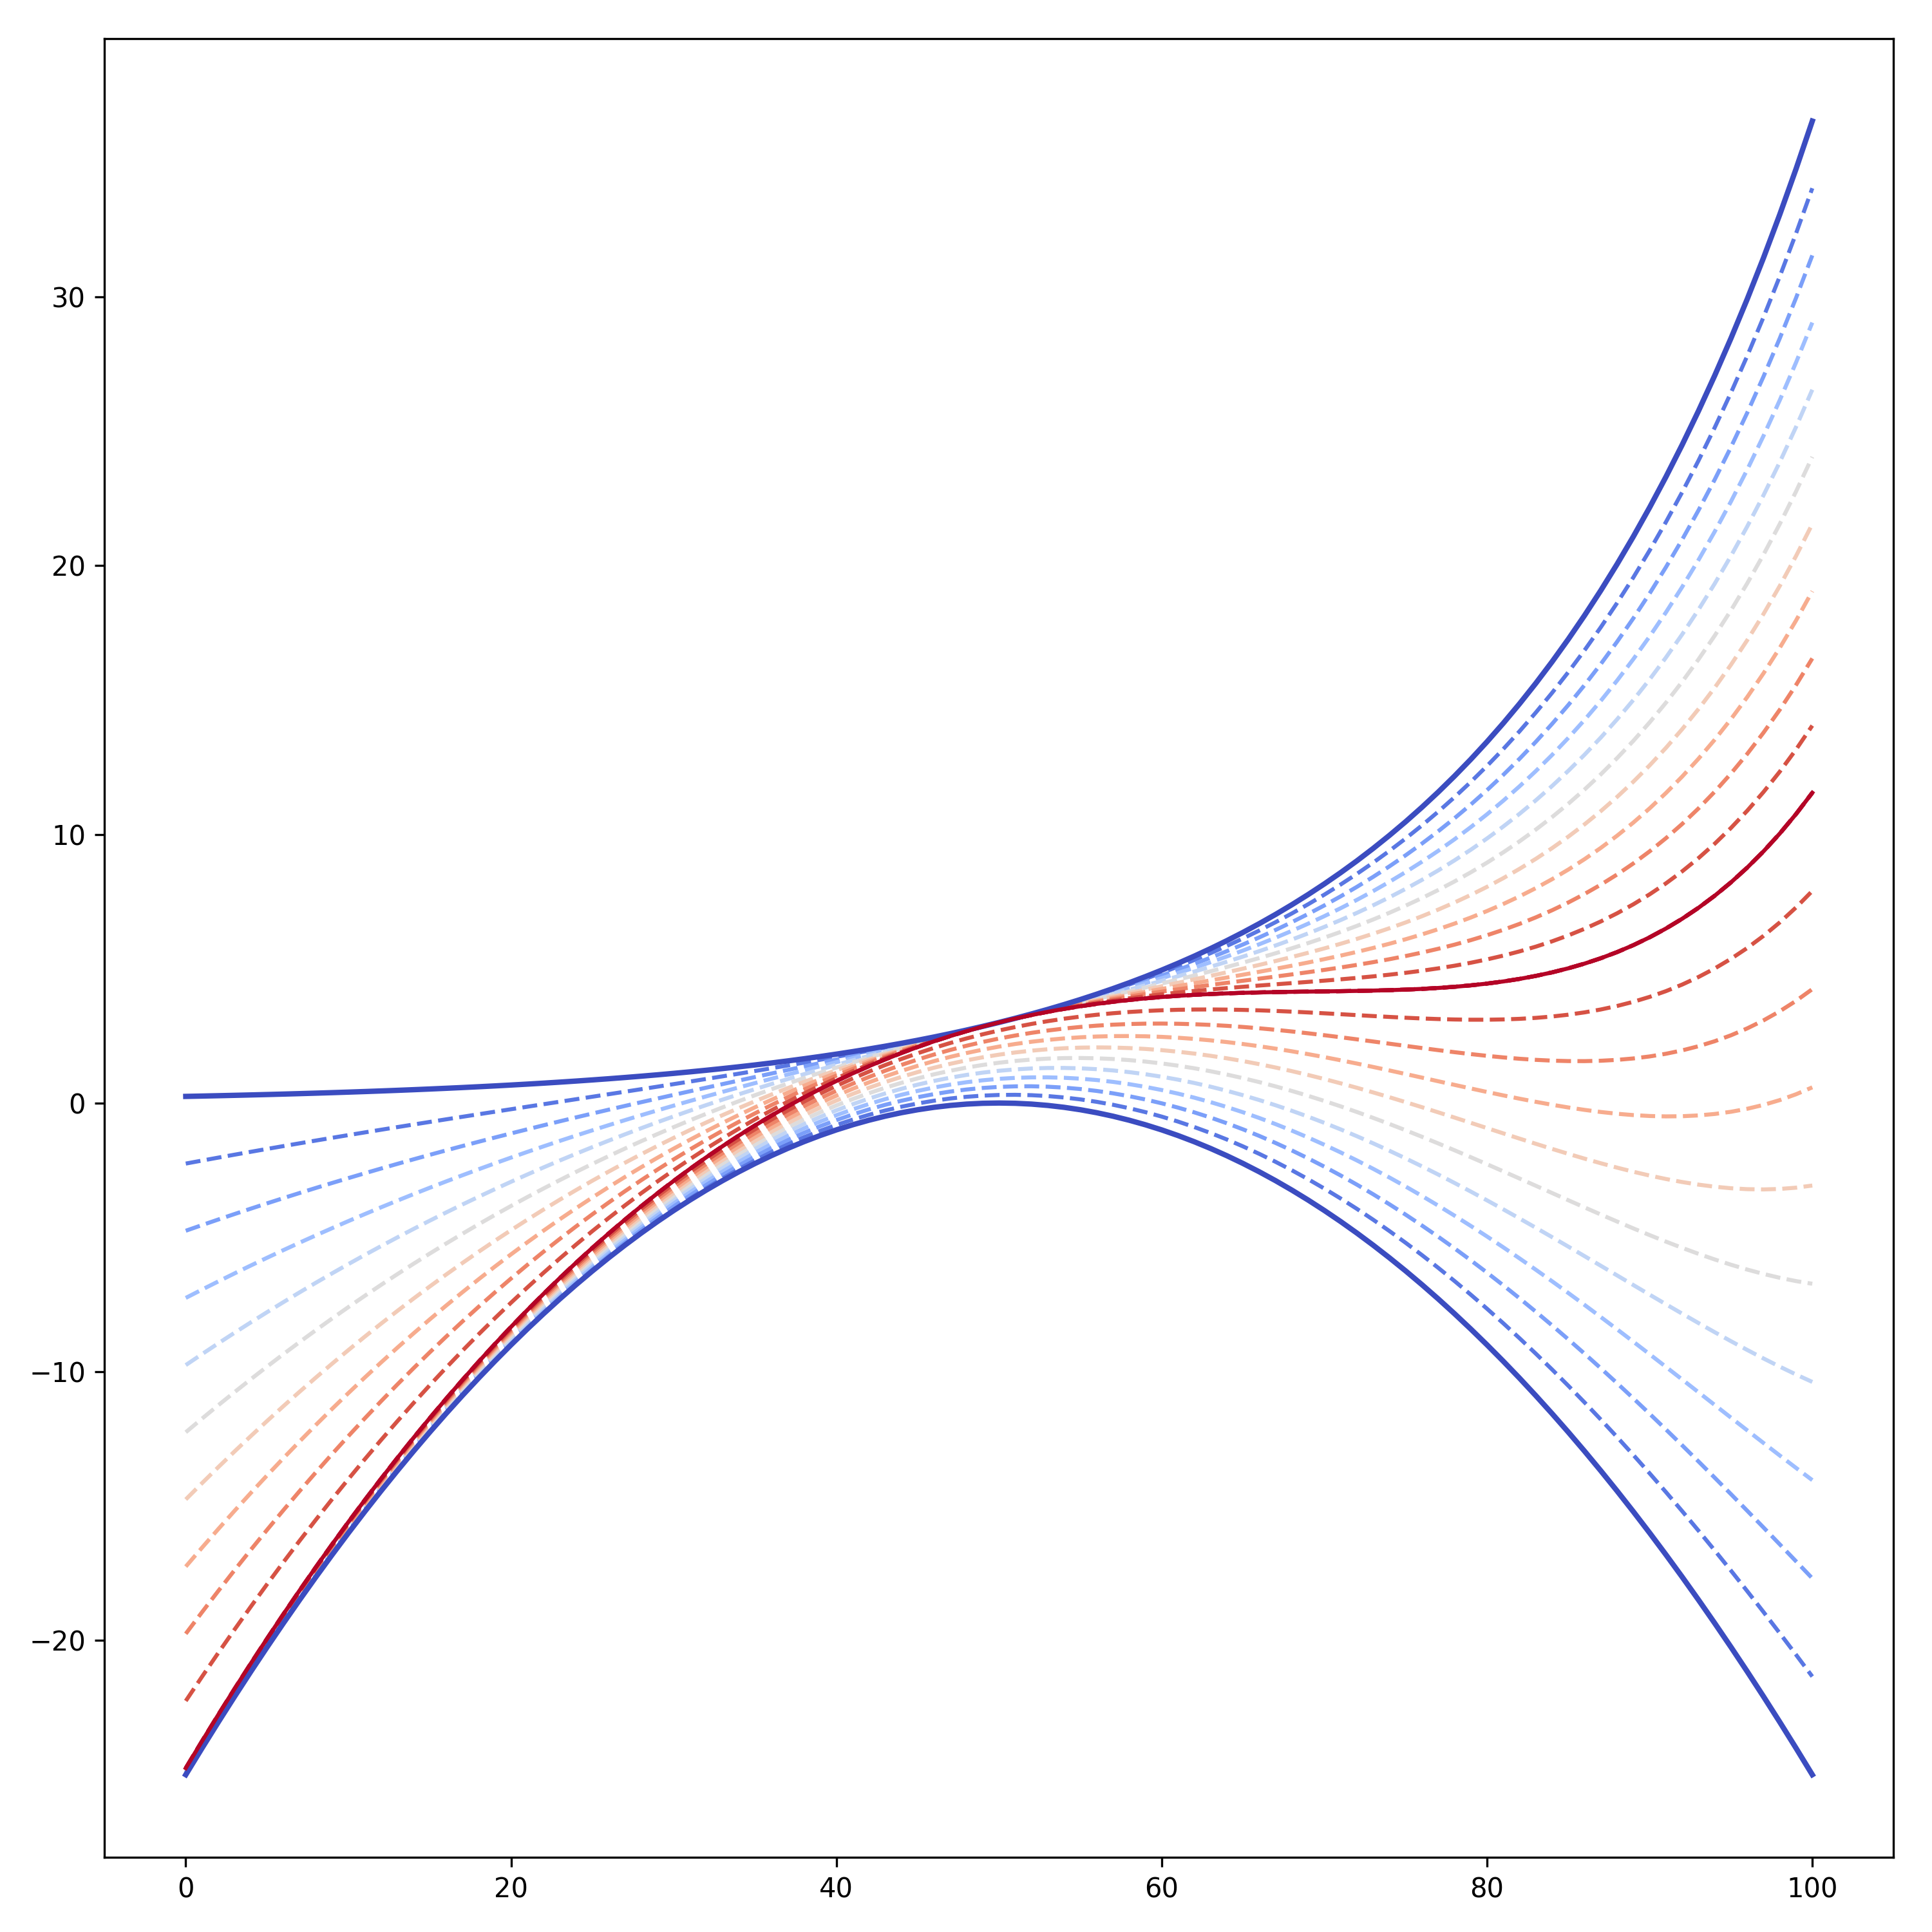
\includegraphics[width=0.65\textwidth]{fig/spline}
    \caption{Example of how two non-linear splines can be added together to create new functions. The thick blue lines are an exponential spline and a polynomial spline. The thick red line is the new function generated by equal weighting of the two splines. The dashed lines represent intermediate weighting values.}
    \label{fig:fancy_spline}
\end{figure}

The simplest and perhaps most common method of choosing splines is to manually apply non-linear functions to an input using available domain knowledge. A simple example of this approach is the introductory physics exercise of applying a quadratic spline to the displacement of a falling object to determine its acceleration from gravity. While effective, this approach is heavily labor intensive, requires significant domain knowledge, and is not guaranteed to be optimal unless there is some strong theoretical foundation for the spline choice. 

A better option is to use machine learning to fit the spline using a special type of function known as a \textit{b-spline} \citep{deBoor2006ASplines}. B-splines, short for \textit{open uniform quadratic basis splines}, are a cheap and effective method of fitting somewhat arbitrary one-dimensional functions. An extension of bézier curves, b-splines use polynomials to smoothly interpolate the values between a set of control points known as \textit{knots}. Each section of the b-spline employs a set of overlapping quadratic bézier curves defined over a small subset of the domain. All knots are equidistant from one another (uniform) and additional knots are added on the ends to force the function to go all the way to the edge of the data (open). By weighting each of these piece-wise curves, we can fit a smooth non-linear approximation of the underlying data.

\begin{figure}[t]
    \centering
    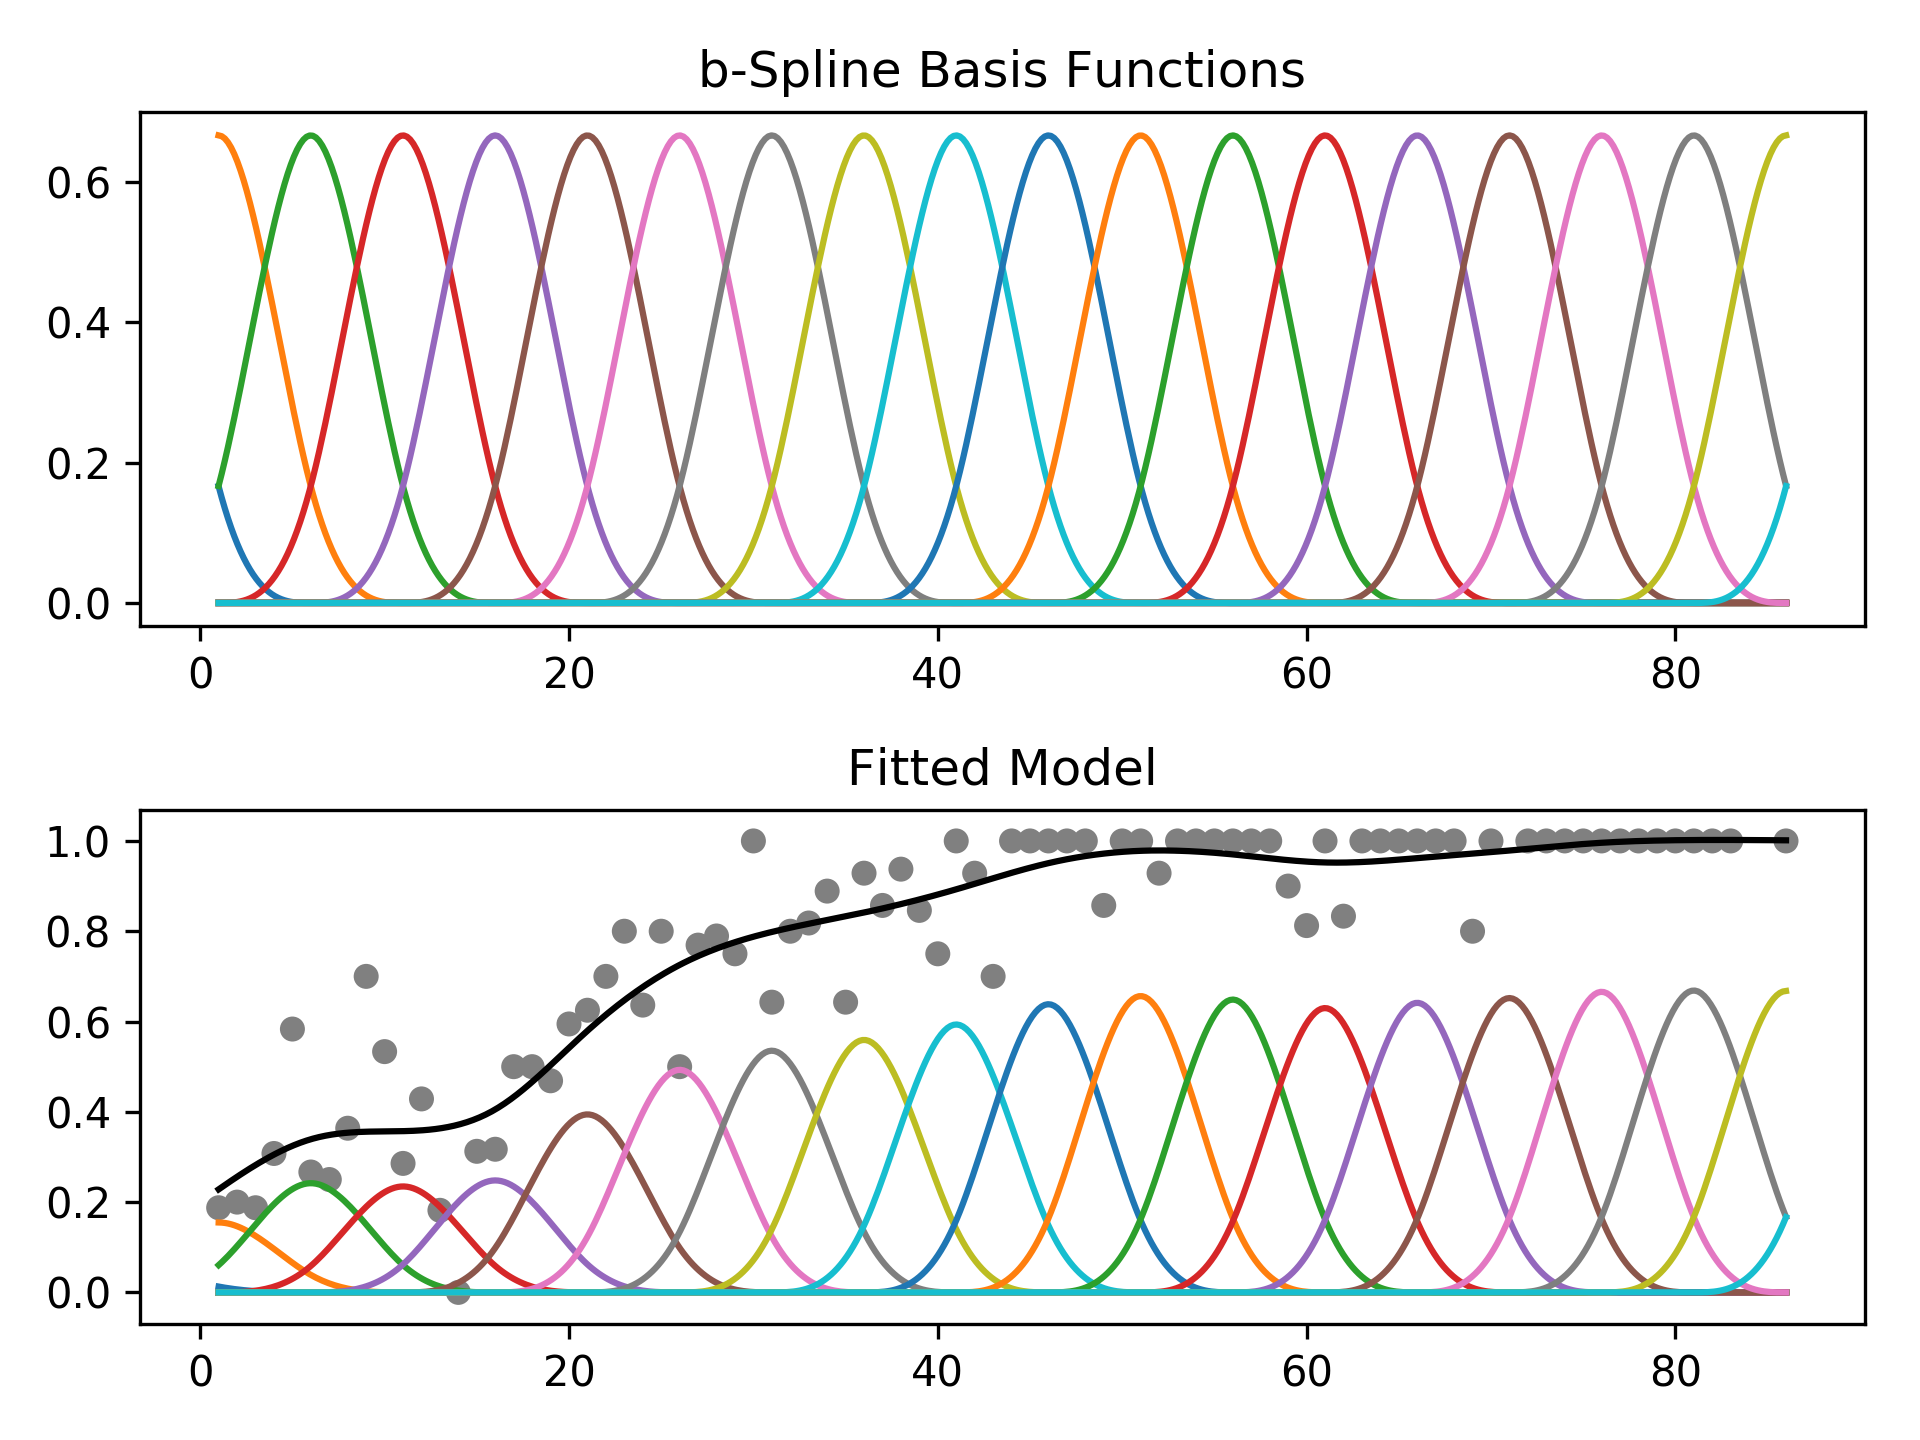
\includegraphics[width=0.65\textwidth]{fig/pygam_basis}
    \caption{Example of how b-splines can be used to smoothly approximate a non-linear univariate function. \citep{Serven2018PyGAM:Python}}
    \label{fig:b-spline}
\end{figure}

GAMs have a number of advantages when compared to other machine learning methods. Unlike simple linear regression and elastic nets, GAMs have non-linear predictive power, allowing them to be used on a wider range of problems. However, unlike random forests and neural networks, GAMs are highly interpretable. By computing the splines, weighting them, and summing them together, \update{it becomes possible to} visualize how each input affects the output. See for instance, how a combination of b-splines combines to form an interpretable non-linear function in Figure \ref{fig:b-spline}.

The output of a GAM can be expressed as a weighted sum of one-dimensional non-linearities (equation \ref{eq:gam}). Because there are no joint terms, these plots describe the complete behavior of the model. This is a useful feature where model interpretability is paramount, as it can provide information about how the model works and prevent errors in unforeseen edge cases or changing input spaces.

\begin{equation}
    \label{eq:gam}
    g(y) = f_1(w_1 x_1) + f_2(w_2 x_2) + ... + f(w_n x_n)
\end{equation}


While extremely useful in high-interpretability situations, GAMs have several drawbacks that have slowed widespread adoption in the machine learning community. First, they are not a universal function approximator, as they cannot handle arbitrary joint functions of the inputs. Second, the splines are often difficult to tune, requiring specific domain knowledge to correctly fit in certain problems.

Despite heavy support in the statistical language, R, there is little support for GAMs in other languages. Python's leading GAM package, pyGAM \citep{Serven2018PyGAM:Python}, is less supported and less frequently used when compared to other important machine learning packages like TensorFlow \citep{Allaire2019RTensorFlow} and SciKit-Learn \citep{Pedregosa2011Scikit-learn:Python}. 

However, what if we were to rebuild the GAM principles in modern machine learning frameworks like TensorFlow? Could neural networks be used to help solve the spline issues, and could we improve support for the method by piggybacking on the development of better supported frameworks?
